\documentclass[11pt]{impeart}

% The manual deliberately applies a global house style.  Ordinary documents
% should normally use \UseFont without a mode or the template `fonts` key.
\UseFont{libertinus}[global]
\setmonofont[
  BoldFont=lmmonolt10-bold.otf,
  ItalicFont=lmmono10-italic.otf,
  BoldItalicFont=lmmonolt10-boldoblique.otf
]{lmmono10-regular.otf}
\UseFeatures{hyperlinks,tables}

\usepackage{catchfile}
\usepackage{metalogo}
\usepackage{pdfpages}

\IfFileExists{VERSION}
  {\CatchFileEdef{\IMPEVersion}{VERSION}{\endlinechar=-1\relax}}
  {\PackageError{impe-manual}
     {Required staged resource VERSION is missing}
     {Run scripts/build_manual.ps1 from the repository root.}}

% Keep the generated manual reproducible when SOURCE_DATE_EPOCH is fixed.
\ifdefined\XeTeXversion
  \special{pdf:trailerid [(IMPE-\IMPEVersion-manual-en)(IMPE-\IMPEVersion-manual-en)]}
\else\ifdefined\pdftrailerid
  \expandafter\pdftrailerid\expandafter{IMPE-\IMPEVersion-manual-en}
\fi
\fi

\title{IMPE \LaTeX{} System}
\subtitle{User Manual}
\author{YANG Sikai}
\date{Version \IMPEVersion}

\newcommand{\IMPERepo}{https://github.com/KelvinYangBK67/IMPE-LaTeX-System}
\newcommand{\IMPEIssues}{https://github.com/KelvinYangBK67/IMPE-LaTeX-System/issues}
\newcommand{\IMPEShowcaseURL}{https://github.com/KelvinYangBK67/IMPE-LaTeX-System/blob/main/_showcase/main.pdf}

\begin{document}

\maketitle

\begin{center}
\small English reference edition
\end{center}

\tableofcontents

\section{Introduction}

IMPE stands for \emph{Integrated Multilingual Publishing Environment}.
The IMPE \LaTeX{} System is a modular document system for \XeLaTeX{} designed
for workflows in which document layout, optional functionality, font selection,
and multilingual typesetting should be reusable rather than reconstructed in
the preamble of every document.  The expanded name describes the system's main
goal: to provide one integrated publishing environment for documents that may
combine multiple languages, writing systems, layouts, and functional modules.

The system grew out of multilingual document work in which a conventional
preamble quickly became difficult to maintain.  A document might need a stable
page design, a Latin text family, CJK support, one or more historical scripts,
script-specific shaping, bibliography support, images, tables, and different
settings for articles, books, and slides.  None of these tasks is unusual by
itself, but the combination tends to produce repeated setup code and a growing
number of document-specific exceptions.

IMPE addresses this by separating the system into reusable parts.  From the
user's point of view, the most important distinction is between \emph{layouts},
\emph{fonts}, and \emph{features}.  A layout describes the principal visual
organization of a document.  Font families provide global or local font
behavior, including script-aware routing where necessary.  Features provide
optional functionality such as mathematics, hyperlinks, citations, tables, or
images.  These parts can be selected independently or combined through one
unified template interface.

The normal use of IMPE is intentionally short.  A wrapper class can establish a
sensible document layout and a default global font setup, after which a user
loads only the additional families or features required by the document.  When
more explicit control is wanted, the same components can be declared in a
single \verb|\UseTemplateSet| call.

\XeLaTeX{} is the primary document engine for IMPE.  This choice allows the system
to rely on Unicode text, OpenType fonts, \texttt{fontspec}, and \XeTeX{}'s
inter-character mechanisms while retaining the familiar \LaTeX{} document model.
Some specialized internal routes may invoke other engines where a particular
script or renderer requires them, but ordinary IMPE documents are intended to
be compiled with \XeLaTeX{}.

This manual is a user-oriented introduction rather than an exhaustive API
reference.  Detailed subsystem documentation is maintained separately in the
repository under \texttt{docs/}.  In particular, the font, layout, feature, and
system documents describe registration fields and implementation details that
would be unnecessarily repetitive here.  This English manual is the reference
edition: translated manuals should follow its structure and technical content.

A visual survey of the system is available in the project showcase at
\href{\IMPEShowcaseURL}{the IMPE showcase PDF}.  The same showcase is also
reproduced in Appendix~\ref{app:showcase}; the repository build stages that PDF
beside the manual source before compilation.  It is intended to demonstrate
the range of scripts, writing directions, layouts, and feature combinations
that motivated the system.

\section{Installation}

\subsection{Distribution forms}

IMPE is prepared in three distribution forms, each intended for a different
use case.

The \emph{CTAN-oriented distribution} contains the portable runtime and public
documentation without the private or locally maintained font library.  This is
the form intended for standard \TeX{} distribution.  The \emph{core distribution}
contains the same system logic for users who prefer to install IMPE directly
from a release and manage fonts separately.  The \emph{full distribution} may
add a prepared local font library, subject to the redistribution status of the
individual fonts.

The distinction is deliberate.  IMPE itself is a document system; a large font
collection is not part of the logical core of the package.  Keeping the two
separate makes the runtime portable and allows different machines or users to
supply different font libraries without modifying the framework.

\subsection{Installed location}

A direct installation places the package in the user's TEXMF tree under

\begin{verbatim}
tex/latex/impe/
\end{verbatim}

so that the package and wrapper classes are available through the normal \TeX{}
search path.  The canonical public entries are

\begin{verbatim}
impe.sty
impeart.cls
impebook.cls
impereport.cls
impebeamer.cls
\end{verbatim}

with corresponding \texttt{\_zh} wrapper classes for Chinese-oriented document
defaults.  Compatibility entries using the earlier \texttt{next*} names are
also installed; see Section~\ref{sec:compatibility}.

When using a direct IMPE release, the supplied installer can be used to copy the
runtime into the user TEXMF tree.  A release archive may provide the usual
Windows entry point

\begin{verbatim}
install.bat
\end{verbatim}

The launcher delegates to \texttt{install.ps1}; advanced callers may invoke
that script with their host's normal script runner.

Users installing through a \TeX{} distribution do not need the repository-side
installer; package discovery is handled by the \TeX{} distribution in the usual
way.

\subsection{Font resources and local configuration}

The source repository does not track the full local font library.  In a local
or full installation, catalogued font files are normally resolved below an
\texttt{assets/fonts/} root.  A different location can be selected without
editing the package itself.

The preferred persistent mechanism is \texttt{impe.local.tex}.  A local setup
may, for example, contain

\begin{verbatim}
\SetCatalogFontRoot{D:/Fonts/IMPE}
\end{verbatim}

with the path adjusted to the local machine.  The same command can also be used
from a document when a one-off override is more appropriate.  Core and CTAN
installations remain usable without a private font collection; only document
features that request unavailable local font files will, naturally, require
those resources to be supplied.

\subsection{A quick installation check}

After installation, the following file should compile with \XeLaTeX{} on a system
with Libertinus available:

\begin{verbatim}
\documentclass{impeart}
\UseFont{libertinus}

\begin{document}
\LIB{IMPE is ready.}
\end{document}
\end{verbatim}

If this succeeds, the canonical wrapper class, package entry, and automatic
font-loading interface are visible to \TeX{}.

\section{Quick Start}

The simplest IMPE workflow is to choose a wrapper class, select any desired
font family or feature, and write the document normally.  IMPE does not replace
ordinary \LaTeX{} document structure; it provides a reusable setup layer around
it.

A small article can therefore look like this:

\begin{verbatim}
\documentclass[11pt]{impeart}

\UseFont{libertinus}
\UseFeatures{math,hyperlinks}

\title{A Sample Document}
\subtitle{Typeset with IMPE}
\author{Author Name}

\begin{document}

\maketitle

\section{Introduction}
\LIB{Hello, world.}

\end{document}
\end{verbatim}

The class already supplies the normal English article layout and base font.
The mode-free \verb|\UseFont{libertinus}| call follows that family's registered
automatic behavior, applying its global stack and making its local \verb|\LIB|
command available, while \verb|\UseFeatures| activates two optional feature
modules.  The rest is ordinary \LaTeX{}.

For a document whose setup is better expressed as a single declaration, the
same idea can be written through \verb|\UseTemplateSet|:

\begin{verbatim}
\documentclass{impeart}

\UseTemplateSet{
  fonts = {libertinus},
  features = {math,hyperlinks}
}
\end{verbatim}

A template set may also choose a layout and additional font families.  In
practice, wrapper classes already supply a suitable default layout, so most
documents only state the settings that differ from those defaults.

IMPE can also be loaded as a package underneath a standard \LaTeX{} class:

\begin{verbatim}
\documentclass{article}
\usepackage{impe}

\UseTemplateSet{
  layout = en_doc,
  fonts = {cmu,libertinus},
  features = {hyperlinks}
}
\end{verbatim}

This form is useful when the underlying class must remain explicit or when every
IMPE component should be selected manually.  The wrapper classes and the raw
package use the same underlying system.


\section{Ready-to-use Templates}

The repository includes a small collection of starter projects under
\texttt{templates/}.  These are intended for actual writing rather than for
regression testing or internal demonstration.  In contrast, the files under
\texttt{examples/} are primarily debugging and audit material.

The current starter templates are:

\begin{description}
  \item[\texttt{article\_en/}] English article starter using \texttt{impeart}.
  \item[\texttt{article\_zh/}] Chinese article starter using \texttt{impeart\_zh}.
  \item[\texttt{book\_en/}] English book starter using \texttt{impebook}.
  \item[\texttt{book\_zh/}] Chinese book starter using \texttt{impebook\_zh}.
  \item[\texttt{beamer\_en/}] English presentation starter using \texttt{impebeamer}.
  \item[\texttt{beamer\_zh/}] Chinese presentation starter using \texttt{impebeamer\_zh}.
\end{description}

Each template follows the installed-package style and contains realistic
metadata, sectioning, and body structure, together with representative table,
figure, or slide material where appropriate.  A new project can therefore begin
by copying the nearest template directory and editing the document contents
instead of reconstructing a preamble from scratch.

The templates deliberately use the canonical \texttt{impe*} entry points.  They
are examples of normal user-facing practice, whereas repository-local
\texttt{examples/} may use paths or fixtures intended only for development and
regression testing.

\section{Document Classes and Public Entry Points}

\subsection{Wrapper classes}

IMPE provides wrapper classes for the four principal document forms used by the
system:

\begin{description}
  \item[\texttt{impeart}] English-oriented article wrapper.  Its normal layout
    is \texttt{en\_doc} and its default global family is \texttt{cmu}.
  \item[\texttt{impebook}] English-oriented book wrapper.  Its normal layout
    is \texttt{en\_book} and its default global family is \texttt{cmu}.
  \item[\texttt{impereport}] English-oriented report wrapper.  It uses the
    \texttt{en\_doc} layout and \texttt{cmu} by default.
  \item[\texttt{impebeamer}] Presentation wrapper.  It selects the
    \texttt{beamer} layout and \texttt{cmu} by default.
\end{description}

Chinese-oriented counterparts are provided as \texttt{impeart\_zh},
\texttt{impebook\_zh}, \texttt{impereport\_zh}, and
\texttt{impebeamer\_zh}.  These select the corresponding Chinese document
settings and include \texttt{shanggu} in the default global font configuration
alongside \texttt{cmu}.  The distinction is a default configuration, not a
restriction on what languages may appear in the document.

Unknown class options are passed through to the underlying standard class.  A
normal option such as

\begin{verbatim}
\documentclass[12pt,twoside]{impeart}
\end{verbatim}

therefore continues to control the underlying \texttt{article} class in the
usual way.

\subsection{Using \texttt{impe.sty} directly}

The wrapper classes are conveniences rather than separate implementations.  A
user may instead keep a standard class and load

\begin{verbatim}
\usepackage{impe}
\end{verbatim}

followed by an explicit layout, font, and feature configuration.  This is the
recommended route when the document class is supplied by a journal, publisher,
or another package and should not be replaced by an IMPE wrapper.

\subsection{Titles and subtitles}

IMPE supports \verb|\subtitle{...}| alongside the standard \verb|\title| and
\verb|\author| commands.  Wrapper classes apply their own title-block defaults,
while the ordinary \LaTeX{} title mechanism remains recognizable.  A typical
preamble is simply

\begin{verbatim}
\title{Main Title}
\subtitle{A More Specific Description}
\author{Author Name}
\end{verbatim}

followed by \verb|\maketitle| in the document body.

\section{The Template Model}

\subsection{Four setup keys}

The principal unified command is \verb|\UseTemplateSet|.  Its public setup
model is intentionally small:

\begin{verbatim}
\UseTemplateSet{
  layout = <preset>,
  fonts = {<families>},
  globalfonts = {<families>},
  features = {<features>}
}
\end{verbatim}

The four keys have different roles.

\begin{description}
  \item[\texttt{layout}] selects a public layout preset appropriate to the
    active document class.
  \item[\texttt{fonts}] loads families through their registered automatic
    behavior.  This is the normal choice: a family may define a local command,
    apply a document-wide font, or install range-specific routing.
  \item[\texttt{globalfonts}] explicitly forces the listed families through
    their global mode or global routing path.
  \item[\texttt{features}] loads optional functional modules.
\end{description}

\texttt{mainfonts} is accepted as an alias of \texttt{globalfonts}; both keys
are explicit global overrides rather than the normal automatic interface.

The template interface is not a requirement that every document declare all
four keys.  Its purpose is to provide one predictable place where a complete
configuration \emph{can} be expressed.  Wrapper classes already apply their
own layout and global-font defaults; specifying only an additional feature list
is therefore perfectly normal.

\subsection{Single-purpose shortcuts}

For documents that do not need a full template declaration, IMPE provides
public shortcuts corresponding to the individual subsystems:

\begin{verbatim}
\UseLayout{en_doc}
\UseLayouts{...}

\UseFont{libertinus}
\UseFonts{arabic,tibetan}

\UseFont{libertinus}[global]
\UseLocalFonts{arabic,tibetan} % explicit local override
\UseGlobalFonts{libertinus}    % explicit global override

\UseFeature{hyperlinks}
\UseFeatures{math,hyperlinks,tables}
\end{verbatim}

The mode-free font forms are the recommended shortcuts for ordinary use.  The
local and global aliases remain useful when a document intentionally overrides
a family's registered behavior.  The unified and single-purpose interfaces are
two views of the same public model rather than competing configuration systems.

\subsection{Composition instead of monolithic templates}

An IMPE template is deliberately not one indivisible style file.  A layout can
be reused with different font choices, the same feature set can be used in an
article or book, and a script-specific font family can be added without
changing unrelated document functionality.  This composition is the central
design principle behind the public interface.

For example, the following declarations describe two quite different documents
without requiring two unrelated preamble templates:

\begin{verbatim}
% English article
\UseTemplateSet{
  layout = en_doc,
  fonts = {libertinus},
  features = {math,hyperlinks}
}

% Chinese book with additional script support
\UseTemplateSet{
  layout = zh_book,
  fonts = {cmu,shanggu,sanskrit,tibetan},
  features = {citations,index,hyperlinks}
}
\end{verbatim}

The second example only states the families and features it needs; the internal
font and layout subsystems remain responsible for the implementation details.

\section{Fonts, Script Routing, and Multilingual Typesetting}

\subsection{Font families as registered capabilities}

IMPE does not treat a font name as merely a replacement for \verb|\rmfamily|.
Font families are registered in a central catalog with the information needed
to use them correctly: available faces, paths or system font names, OpenType
script and language settings, local command metadata, global routing behavior,
and, where necessary, a specialized layout or rendering route.

This model allows a simple Latin family and a complex-script family to share
the same public loading interface even when their internal requirements are
very different.  The common abstraction is the \emph{registered family}, not a
claim that every writing system is implemented identically.

\subsection{Automatic, global, and local loading}

For ordinary use, load a family without a mode.  IMPE then follows the
family's registered behavior, which may be local, global, or range-specific.
The \texttt{fonts} template key applies the same automatic rule to a list.

A \emph{global} family participates in document-wide font selection.  For a
normal Latin family this can mean replacing the main roman, sans-serif, and
monospaced channels.  For a script-specific family it can instead mean taking
responsibility only for selected Unicode ranges while leaving Latin, Han, and
other scripts untouched.

A \emph{local} family is loaded for explicit use.  Local selection is useful
when a particular passage requires a specific script font, a regional glyph
form, or an editorially chosen typeface without changing the document-wide
routing.

Families are loaded through, for example,

\begin{verbatim}
\UseFont{libertinus}
\UseFonts{sanskrit,tibetan,arabic}

\UseFont{libertinus}[global]   % deliberate global override
\UseLocalFonts{sanskrit}       % deliberate local override
\end{verbatim}

or through the corresponding keys in \verb|\UseTemplateSet|.  The
\verb|\UseGlobalFont(s)| and \verb|\UseLocalFont(s)| aliases are explicit
overrides, not the default recommendation.  Public commands created for
individual local families are defined by their catalog registrations; the
complete list belongs in the font reference rather than in this introductory
manual.

When an explicit local font command is active, it takes precedence over the
automatic global range router within that scope.  Leaving the local scope
restores the global routing state.  This makes explicit authorial choice
predictable even in a document with extensive automatic script selection.

\subsection{Unicode-range routing}

Some global families are intentionally range-limited.  A Devanagari family,
for example, need not become the Latin main font simply because it is loaded
globally.  IMPE can assign such a family only to the Unicode blocks for which
it is responsible.  Multiple registered families can therefore coexist in one
document without continually replacing one another's text.

This routing is most useful for genuinely multilingual prose: the author writes
Unicode text normally, while IMPE selects the active registered family when the
text enters a configured script range.  Range routing is an aid to font
selection; shaping remains the responsibility of \XeTeX{}, \texttt{fontspec}, and
the OpenType data associated with the selected family.

\subsection{CJK handling}

CJK fonts require a somewhat different route from ordinary Unicode-range
switching.  IMPE uses the xeCJK path for CJK global families, allowing the main,
sans-serif, and monospaced CJK channels to be managed as CJK fonts rather than
as a collection of isolated character switches.

Shared Han ideographs create an additional problem: Unicode alone does not say
whether a Han character in a particular context should use Chinese, Japanese,
or Korean regional glyph conventions.  Automatic routing therefore gives
language-specific scripts such as kana and Hangul their own claims while
leaving shared Han characters on the document CJK family.  When an explicitly
Japanese or Korean Han form is required, a local family command can be used to
make that choice directly.

This distinction is intentional.  Automatic routing should make the common
case convenient without pretending that ambiguous Han characters contain
language information which Unicode does not provide.

\subsection{Shaping and line breaking}

OpenType shaping for ordinary complex scripts is expressed through the
registered script, language, and feature settings of a family.  Indic, Arabic,
and other shaping-sensitive scripts therefore remain ordinary Unicode text at
the document level; IMPE supplies the font configuration needed for the text
engine to shape them correctly.

Some scripts also need line-breaking behavior that is not adequately described
by ordinary spaces.  IMPE includes script-aware handling for cases such as
Sanskrit in Devanagari, Tibetan, and Thai.  The purpose is not to replace the
language's orthography with manual break markers, but to let the font and
behavior layers provide appropriate opportunities while preserving clusters or
script-specific punctuation rules.

Right-to-left behavior is likewise attached to families that require it.  The
public font model remains the same even though the underlying paragraph or
inline behavior differs from a left-to-right Latin family.

\subsection{Vertical and externalized rendering}

A small number of writing systems need more than standard horizontal OpenType
shaping.  IMPE therefore includes a built-in vertical layout route used by
registered vertical families, and it provides an externalized rendering path
for cases where a fragment is more reliably produced as a small auxiliary \TeX{}
document and reinserted as PDF.

Externalized rendering is implemented through a portable \texttt{texlua} helper.  The
helper resolves the requested \TeX{} engine from the system \texttt{PATH}, renders
into an IMPE cache directory, and returns the resulting PDF to the main
document.  The mechanism is kept behind the font registration layer so that a
normal document does not need to manage temporary files or engine paths
manually.

These specialized routes are exceptions at the implementation level, not at
the user-interface level.  They exist precisely so that the public font model
can remain coherent when a script cannot be handled by a simple
\verb|\newfontfamily| declaration.

\subsection{Where to find the complete font reference}

The detailed family catalog, registration syntax, style fallback rules, global
routing model, vertical parameters, externalized backend, and script-specific
notes are maintained in \texttt{docs/FONTS.md}.  Users adding a new family or
investigating font-routing behavior should treat that document as the technical
reference.

\section{Layouts and Features}

\subsection{Layout presets}

Layouts describe document-level presentation.  A public layout preset is a
structured bundle of page geometry, text spacing, header behavior, book
behavior, or slide behavior.  The individual low-level components are internal;
normal documents select the public preset as a whole.

The public presets in IMPE 1.0.0 are:

\begin{description}
  \item[\texttt{en\_doc}] English article/report layout.
  \item[\texttt{zh\_doc}] Chinese article/report layout.
  \item[\texttt{en\_book}] English book/report layout with book-oriented page
    and running-head behavior.
  \item[\texttt{zh\_book}] Chinese book/report counterpart.
  \item[\texttt{beamer}] presentation layout for Beamer documents.
\end{description}

Presets declare which underlying document classes they support.  IMPE checks
that compatibility before applying the preset, so a slide layout is not
silently applied to an article or vice versa.

Wrapper classes select the corresponding layout automatically.  Explicit
selection is useful with raw standard classes or when a report should use a
book-oriented preset:

\begin{verbatim}
\UseLayout{en_book}
\end{verbatim}

The exact component values and geometry are documented in
\texttt{docs/LAYOUTS.md}.

\subsection{Feature modules}

Features are flat, composable modules.  Unlike layouts, they do not have a
second preset layer.  A feature id simply loads the corresponding optional
functionality the first time it is requested; repeated requests are ignored.

The public feature set currently consists of:

\begin{description}
  \item[\texttt{math}] standard mathematics packages, theorem environments,
    and optional math-font selection.
  \item[\texttt{hyperlinks}] hyperlinks, PDF bookmarks, stable destinations,
    and repository hyperlink defaults.
  \item[\texttt{citations}] \texttt{biblatex}/\texttt{biber} citation support
    with selectable citation-style presets.
  \item[\texttt{index}] index generation and IMPE term/index helpers.
  \item[\texttt{tables}] table packages, reusable column types, and table
    environments.
  \item[\texttt{image}] figure, image, and multi-panel helpers.
  \item[\texttt{lists\_envs}] reusable example-block formatting.
  \item[\texttt{headers}] configurable running heads for article-, report-,
    and book-like documents.
\end{description}

A document loads any combination it requires:

\begin{verbatim}
\UseFeatures{math,hyperlinks,tables,image}
\end{verbatim}

or

\begin{verbatim}
\UseTemplateSet{
  features = {citations,index,hyperlinks}
}
\end{verbatim}

\subsection{Mathematics}

The \texttt{math} feature loads the standard AMS-oriented mathematics stack and
defines theorem-like environments including \texttt{theorem}, \texttt{lemma},
\texttt{proposition}, \texttt{corollary}, \texttt{definition},
\texttt{example}, and \texttt{remark}.  Loading a text family does not by itself
force a new math alphabet: Computer Modern mathematics remains the default
unless an explicit math route is selected.

A different math family can be selected before the feature is loaded.  For
example,

\begin{verbatim}
\UseMathFont{libertinus}
\UseFeature{math}
\end{verbatim}

uses Libertinus Math through \texttt{unicode-math}.  Other supported routes and
the exact package stack are listed in \texttt{docs/FEATURES.md}.

\subsection{Citations, indexes, tables, and figures}

The feature modules are designed to provide useful defaults without hiding the
underlying \LaTeX{} ecosystem.  The \texttt{citations} feature, for example, uses
\texttt{biblatex} and \texttt{biber}; documents still use ordinary commands
such as \verb|\addbibresource|, \verb|\textcite|, and
\verb|\printbibliography|.  Citation presets such as APA, GB/T 7714, numeric,
or author--year may be selected before the feature is loaded.

The \texttt{index} feature builds on \texttt{imakeidx} and adds the
\verb|\Term| helper for typesetting and indexing a term together.  The
\texttt{tables} and \texttt{image} features similarly provide convenient
higher-level environments while leaving native \texttt{booktabs},
\texttt{graphicx}, and related commands available.

This is the intended balance throughout the feature system: IMPE should reduce
repetitive setup, not create a private replacement language for ordinary
\LaTeX{}.

\subsection{Headers and hyperlinks}

The \texttt{headers} feature supplies running heads through
\texttt{fancyhdr}.  By default it derives a fixed running title from the first
line of \verb|\title|; \verb|\HeaderTitle{...}| can be used when a shorter form
is preferable.  Article-like documents use section information for the moving
head, while report- and book-like documents use chapter information.

The \texttt{hyperlinks} feature loads \texttt{hyperref} and
\texttt{bookmark} with Unicode-aware PDF settings, hidden link borders, linked
table-of-contents structures, and stable destinations.  Documents may still use
ordinary \verb|\label|, \verb|\ref|, \verb|\href|, and \verb|\url| commands.

For the full list of feature-specific commands and environments, consult
\texttt{docs/FEATURES.md} rather than treating this section as an API catalog.

\section{Compatibility and Migration}\label{sec:compatibility}

IMPE 1.0.0 establishes the \texttt{impe*} names as the canonical public
interface.  New documents should therefore use \texttt{impe.sty},
\texttt{impeart}, \texttt{impebook}, \texttt{impereport},
\texttt{impebeamer}, and their Chinese variants.

Earlier development releases used the \texttt{next*} naming scheme.  Those
entry points remain supported compatibility wrappers in 1.0.0; they are not
deprecated in this release.  Existing documents such as

\begin{verbatim}
\documentclass{nextart}
\usepackage{nextsystem}
\end{verbatim}

can therefore continue to compile against the same underlying implementation.
The compatibility layer exists to preserve old documents, not to define a
parallel set of APIs for new work.

The direct installer also recognizes a managed installation from the 0.1.x
series under \texttt{tex/latex/nextsystem/}.  During migration it installs the
canonical runtime under \texttt{tex/latex/impe/}, migrates recognized local
override files when appropriate, removes files known to belong to the old
managed runtime, and leaves unrelated user-created files or subdirectories in
place.

A legacy \texttt{nextsystem.local.tex} can therefore survive migration without
requiring the old generic runtime filenames to remain visible in the TEXMF
tree.  New local configuration should use \texttt{impe.local.tex}.

No source-level conversion is required merely because a document was written
with the old wrapper names.  Authors may update those names when convenient,
but compatibility is intentionally a runtime concern rather than a forced
migration of every existing document.

\section{Package Structure and Extension Points}

The repository separates public entry points, stable mechanisms, registrations,
specialized implementations, and local resources:

\begin{verbatim}
package/   public package and class entry points
core/      stable subsystem mechanisms
catalog/   public ids and registration data
modules/   extendable or specialized implementations
assets/    local runtime resources such as fonts
scripts/   installation and release tooling
doc/       manual sources
docs/      detailed subsystem documentation
\end{verbatim}

\subsection{The stable core}

The \texttt{core/} layer contains the framework that should not have to change
whenever a new font family, layout preset, or feature is added.  It implements
the font registry and routing machinery, the layout registry and compatibility
checks, the feature loader, and related shared behavior.

This distinction matters for maintenance.  If adding one ordinary OpenType
font requires editing the font-routing engine, or adding one feature requires
changing the generic feature loader, the extension model has failed.  The core
is therefore intentionally separated from the growing catalog of concrete
resources.

\subsection{Catalogs}

The \texttt{catalog/} layer assigns public ids and metadata.  It contains the
central registrations for fonts, layouts, and features.  For many extensions,
this is the correct place to begin.

An ordinary font family that needs only standard \texttt{fontspec} shaping can
usually be expressed entirely as a catalog registration.  Likewise, a public
layout preset is assembled from existing internal components, and a feature id
maps to its implementation module.  Keeping those declarations centralized
makes the public surface auditable without searching through the entire source
tree.

\subsection{Modules}

The \texttt{modules/} layer is reserved for functionality that genuinely needs
its own implementation: feature modules, specialized script support, or
reusable internal layout components.  A new module should therefore represent a
real behavioral extension rather than merely a convenient place to put a font
name.

This rule is particularly important for multilingual support.  Most scripts
should use ordinary OpenType shaping and catalog metadata.  Specialized modules
are appropriate only when the writing system or rendering strategy requires
behavior that the generic core cannot express cleanly.

\subsection{Extending IMPE}

The detailed registration interfaces are intentionally outside the scope of
this user manual.  Developers extending the system should begin with
\texttt{docs/SYSTEM.md} and then consult the relevant subsystem document:
\texttt{docs/FONTS.md}, \texttt{docs/LAYOUTS.md}, or
\texttt{docs/FEATURES.md}.

The general rule is simple: prefer a registration over a new mechanism, and
prefer a specialized module over a change to the stable core when the behavior
is genuinely exceptional.

\section{Further Documentation and Feedback}

This manual is the normal starting point for using IMPE.  The repository
contains more detailed technical documentation for users who need a complete
reference or who want to extend the system.

\begin{description}
  \item[\texttt{docs/SYSTEM.md}] architecture, public entry layers, template
    setup, release model, and extension boundaries.
  \item[\texttt{docs/FONTS.md}] family registration, local and global modes,
    routing, fallback, shaping, writing behavior, vertical support, and
    externalized rendering.
  \item[\texttt{docs/LAYOUTS.md}] public layout presets, compatibility targets,
    and the component model from which presets are built.
  \item[\texttt{docs/FEATURES.md}] public feature ids and the commands,
    environments, package stacks, and compilation requirements supplied by each
    module.
  \item[\texttt{CHANGELOG.md}] changes in published versions.
  \item[Showcase] the full visual showcase is available from the
    \href{\IMPEShowcaseURL}{project repository}.
\end{description}

The project repository is available at

\begin{center}
\href{\IMPERepo}{\texttt{github.com/KelvinYangBK67/IMPE-LaTeX-System}}
\end{center}

Bug reports, feature requests, documentation corrections, portability reports,
and other concrete feedback are welcome through GitHub Issues:

\begin{center}
\href{\IMPEIssues}{\texttt{github.com/KelvinYangBK67/IMPE-LaTeX-System/issues}}
\end{center}

When reporting a typesetting problem, it is useful to include a minimal source
file, the \TeX{} engine and \TeX{} Live version, the IMPE version, and the relevant
font information.  Reports concerning a local or privately supplied font should
also distinguish between a font-coverage problem and an IMPE routing problem
where possible.

The English manual is the authoritative manual text.  Other language editions
may adapt prose and terminology to their own technical conventions, but their
commands, examples, and description of IMPE behavior should remain synchronized
with this edition.



\appendix

\section{Quick Reference}
\label{app:quick-reference}

This appendix summarizes the documented public interface of IMPE 1.0.0.
It is intended for lookup rather than as a replacement for the explanations in
the main text or the detailed subsystem documentation under \texttt{docs/}.
Internal implementation commands, in particular commands beginning with
\texttt{\string\Next...}, are not part of this reference.

\subsection{Recommended font-loading model}

For ordinary use, prefer \texttt{fonts = \{...\}} inside
\texttt{\string\UseTemplateSet} or use \texttt{\string\UseFont\{...\}}
directly.  With no explicit mode, IMPE follows the registered behavior of the
family: it may define a local command, activate a document-wide font, or install
script- or range-specific automatic routing as appropriate.

Use an explicit mode only when that automatic behavior is not what the document
needs:

\begin{verbatim}
\UseFont{sanskrit}          % recommended: registered automatic behavior
\UseFont{sanskrit}[local]   % explicitly local only
\UseFont{sanskrit}[global]  % explicitly global/range-global

\UseTemplateSet{
  fonts = {sanskrit,tibetan,arabic},
  features = {math,hyperlinks}
}
\end{verbatim}

The convenience commands \texttt{\string\UseGlobalFont(s)} and
\texttt{\string\UseLocalFont(s)} express the same explicit distinction.
The \texttt{globalfonts} and \texttt{mainfonts} template keys are likewise
explicit global overrides; they are not the normal replacement for
\texttt{fonts}.

\subsection{Document classes and package entry points}

\begin{longtable}{@{}p{0.31\linewidth}p{0.63\linewidth}@{}}
\toprule
\textbf{Entry point} & \textbf{Purpose} \\
\midrule
\endfirsthead
\toprule
\textbf{Entry point} & \textbf{Purpose} \\
\midrule
\endhead
\texttt{impeart} &
English article wrapper; defaults to \texttt{en\_doc} with CMU as the base global font. \\
\texttt{impeart\_zh} &
Chinese article wrapper; defaults to \texttt{zh\_doc} with CMU and Shanggu. \\
\texttt{impereport} &
English report wrapper; defaults to \texttt{en\_doc}. \\
\texttt{impereport\_zh} &
Chinese report wrapper; defaults to \texttt{zh\_doc}. \\
\texttt{impebook} &
English book wrapper; defaults to \texttt{en\_book}. \\
\texttt{impebook\_zh} &
Chinese book wrapper; defaults to \texttt{zh\_book}. \\
\texttt{impebeamer} &
English Beamer wrapper; defaults to the \texttt{beamer} layout. \\
\texttt{impebeamer\_zh} &
Chinese Beamer wrapper; defaults to the \texttt{beamer} layout with CMU and Shanggu. \\
\texttt{impe.sty} &
Loads IMPE under an ordinary \LaTeX{} class when no wrapper class is desired. \\
\bottomrule
\end{longtable}

The legacy \texttt{next*} package and class names remain compatibility aliases
in version 1.0.0, but new documents should use the canonical \texttt{impe*}
entry points.

\subsection{Core setup commands}

\begin{longtable}{@{}p{0.38\linewidth}p{0.56\linewidth}@{}}
\toprule
\textbf{Command} & \textbf{Purpose} \\
\midrule
\endfirsthead
\toprule
\textbf{Command} & \textbf{Purpose} \\
\midrule
\endhead
\texttt{\string\UseTemplateSet\{...\}} &
Configure layout, fonts, and features in one declaration. \\
\texttt{\string\UseFont\{id\}[mode]} &
Load one registered font family; omit \texttt{mode} for the recommended automatic behavior, or use \texttt{local}/\texttt{global} explicitly. \\
\texttt{\string\UseFonts\{ids\}[mode]} &
Load several registered font families with the same optional mode. \\
\texttt{\string\UseGlobalFont\{id\}} &
Explicitly request the global mode of one family. \\
\texttt{\string\UseGlobalFonts\{ids\}} &
Explicitly request the global mode of several families. \\
\texttt{\string\UseMainFont\{id\}} &
Alias of \texttt{\string\UseGlobalFont}; retained as a document-oriented name. \\
\texttt{\string\UseMainFonts\{ids\}} &
Alias of \texttt{\string\UseGlobalFonts}. \\
\texttt{\string\UseLocalFont\{id\}} &
Explicitly request the local mode of one family. \\
\texttt{\string\UseLocalFonts\{ids\}} &
Explicitly request the local mode of several families. \\
\texttt{\string\UseLayout\{id\}} &
Load one registered layout preset. \\
\texttt{\string\UseLayouts\{ids\}} &
Load several registered layout presets. \\
\texttt{\string\UseFeature\{id\}} &
Load one optional feature module. \\
\texttt{\string\UseFeatures\{ids\}} &
Load several optional feature modules. \\
\texttt{\string\SetCatalogFontRoot\{path\}} &
Override the root directory from which catalogued font files are resolved. \\
\texttt{\string\subtitle\{text\}} &
Set the document subtitle used by the IMPE title block. \\
\texttt{\string\HeaderTitle\{text\}} &
Override the fixed title used by the \texttt{headers} feature. \\
\texttt{\string\HeaderStyle\{style\}} &
Choose the header style; documented values are \texttt{running} and \texttt{title}. \\
\bottomrule
\end{longtable}

\subsection{Template-set keys}

\begin{longtable}{@{}p{0.23\linewidth}p{0.69\linewidth}@{}}
\toprule
\textbf{Key} & \textbf{Meaning} \\
\midrule
\endfirsthead
\toprule
\textbf{Key} & \textbf{Meaning} \\
\midrule
\endhead
\texttt{layout} &
Select one public layout preset. \\
\texttt{fonts} &
Load one or more registered families using their automatic registered behavior; this is the recommended key for normal font loading. \\
\texttt{globalfonts} &
Explicitly force the listed families through their global mode or global routing path. \\
\texttt{mainfonts} &
Alias of \texttt{globalfonts}. \\
\texttt{features} &
Load one or more optional feature modules. \\
\bottomrule
\end{longtable}

\subsection{Public layout identifiers}

\begin{longtable}{@{}p{0.23\linewidth}p{0.69\linewidth}@{}}
\toprule
\textbf{ID} & \textbf{Purpose} \\
\midrule
\endfirsthead
\toprule
\textbf{ID} & \textbf{Purpose} \\
\midrule
\endhead
\texttt{en\_doc} &
English article/report layout with A4 geometry and English text spacing. \\
\texttt{zh\_doc} &
Chinese article/report layout with A4 geometry and Chinese text spacing. \\
\texttt{en\_book} &
English book/report layout with book geometry, running heads, and right-hand chapter openings. \\
\texttt{zh\_book} &
Chinese book/report layout with book geometry, Chinese text spacing, running heads, and right-hand chapter openings. \\
\texttt{beamer} &
Presentation layout with the IMPE Beamer typography and navigation setup. \\
\bottomrule
\end{longtable}

\subsection{Public feature identifiers}

\begin{longtable}{@{}p{0.23\linewidth}p{0.69\linewidth}@{}}
\toprule
\textbf{ID} & \textbf{Purpose} \\
\midrule
\endfirsthead
\toprule
\textbf{ID} & \textbf{Purpose} \\
\midrule
\endhead
\texttt{math} &
Load the IMPE mathematics stack and theorem environments. \\
\texttt{hyperlinks} &
Load hyperlinking, PDF bookmarks, linked headings, and bidirectional footnote links. \\
\texttt{citations} &
Load \texttt{biblatex}/\texttt{csquotes} citation support and IMPE citation-style helpers. \\
\texttt{index} &
Load index support and the \texttt{\string\Term} helper. \\
\texttt{tables} &
Load the table stack, column types, and IMPE table environments. \\
\texttt{image} &
Load image, caption, and panel-figure helpers. \\
\texttt{lists\_envs} &
Load the \texttt{ExampleBlock} display environment. \\
\texttt{headers} &
Load configurable running heads for article-, report-, and book-like documents. \\
\bottomrule
\end{longtable}

\subsection{Feature-specific commands and values}

\begin{longtable}{@{}p{0.51\linewidth}p{0.43\linewidth}@{}}
\toprule
\textbf{Command or setting} & \textbf{Purpose / documented values} \\
\midrule
\endfirsthead
\toprule
\textbf{Command or setting} & \textbf{Purpose / documented values} \\
\midrule
\endhead
\texttt{\string\UseMathFont\{value\}} &
Choose the mathematics font route before loading \texttt{math}: \texttt{auto}, \texttt{libertinus}, \texttt{newcm}, \texttt{mlmodern}, or another font name passed to \texttt{\string\setmathfont}. \\
\texttt{\string\UseCitationStyle\{value\}} &
Choose a citation preset before loading \texttt{citations}: \texttt{APA}, \texttt{GB}, \texttt{numeric}, or \texttt{author-year}. \\
\texttt{\string\SetCitationBiblatexOptions\{...\}} &
Replace the effective \texttt{biblatex} option list before loading \texttt{citations}. \\
\texttt{\string\HeaderTitle\{text\}} &
Set a short fixed title for running heads. \\
\texttt{\string\HeaderStyle\{value\}} &
Select \texttt{running} or \texttt{title}. \\
\texttt{\string\IndexTitle} &
Optional index-title override, defined before loading \texttt{index}. \\
\texttt{\string\Term[options]\{display\}[description]} &
Print a bold term and index its first occurrence; options include \texttt{sort}, \texttt{key}, and \texttt{parentheses}. \\
\texttt{\string\TablesSetup} &
Apply or re-apply the IMPE table setup. \\
\texttt{\string\Panel} &
Insert one panel inside \texttt{PanelFigure} or \texttt{PanelFigure*}. \\
\texttt{\string\TemplateFigurePaths} &
Configure the default search paths used by the image feature. \\
\texttt{\string\OneImageDefaultWidth} &
Set the default width for \texttt{OneImage}. \\
\texttt{\string\OneImageMaxHeight} &
Set the maximum default image height for \texttt{OneImage}. \\
\texttt{\string\OneImageDefaultPlacement} &
Set the default float placement for \texttt{OneImage}. \\
\texttt{\string\PanelDefaultCols} &
Set the default number of columns used by panel figures. \\
\texttt{\string\PanelDefaultHeight} &
Set the default panel height. \\
\texttt{\string\PanelDefaultMode} &
Set the default panel layout mode. \\
\texttt{\string\PanelDefaultPlacement} &
Set the default float placement for panel figures. \\
\bottomrule
\end{longtable}

Standard commands provided directly by packages loaded by a feature---for
example \texttt{\string\addbibresource}, \texttt{\string\printbibliography},
\texttt{\string\printindex}, or the \texttt{booktabs} rule commands---retain
their normal package syntax and are not redefined by IMPE.

\subsection{Public environments and table column types}

\begin{longtable}{@{}p{0.37\linewidth}p{0.57\linewidth}@{}}
\toprule
\textbf{Name} & \textbf{Purpose} \\
\midrule
\endfirsthead
\toprule
\textbf{Name} & \textbf{Purpose} \\
\midrule
\endhead
\texttt{theorem}, \texttt{lemma}, \texttt{proposition}, \texttt{corollary} &
Numbered theorem-like environments provided by the \texttt{math} feature. \\
\texttt{definition}, \texttt{example}, \texttt{remark} &
Additional theorem-style environments provided by the \texttt{math} feature. \\
\texttt{TableInlineFit} &
Compact table environment intended to fit an inline table to the available width. \\
\texttt{TableLong} &
Long-table environment for material that may span pages. \\
\texttt{TableBook}, \texttt{TableBookX} &
Book-style table environments. \\
\texttt{TableBookNotes} &
Book-style table environment with notes. \\
\texttt{NiceBooktable}, \texttt{NiceBooktableX}, \texttt{NiceBooktableNotes} &
Alternative book-style table helpers provided by the \texttt{tables} feature. \\
\texttt{L}, \texttt{C}, \texttt{R} &
Ragged-right, centered, and ragged-left \texttt{tabularx} columns. \\
\texttt{P\{w\}}, \texttt{M\{w\}}, \texttt{B\{w\}} &
Fixed-width paragraph columns with ragged-right, centered, and ragged-left alignment. \\
\texttt{OneImage} &
Single-image figure; becomes inline rather than floating under Beamer. \\
\texttt{OneImageInline} &
Centered non-floating image. \\
\texttt{PanelFigure} &
Captioned multi-panel figure with subcaptions outside Beamer. \\
\texttt{PanelFigure*} &
Uncaptioned multi-panel figure. \\
\texttt{ExampleBlock} &
Indented italic display block for examples, quotations, linguistic data, or teaching material. \\
\bottomrule
\end{longtable}

\subsection{Registered font-family identifiers}

The table below lists the font-family IDs accepted by
\texttt{\string\UseFont} in IMPE 1.0.0.  The \textbf{Auto} column summarizes
what a mode-less \texttt{\string\UseFont\{id\}} normally activates:

\begin{description}
  \item[\texttt{G}] document-global family;
  \item[\texttt{L}] local family/command;
  \item[\texttt{L+G}] local access plus full document-global activation;
  \item[\texttt{L+R}] local access plus automatic script- or range-limited global routing.
\end{description}

The automatic route is the recommended interface.  An explicit
\texttt{[local]} or \texttt{[global]} request deliberately bypasses part of
that automatic decision and should therefore be used only when required.

\begin{longtable}{@{}p{0.30\linewidth}p{0.11\linewidth}p{0.18\linewidth}p{0.31\linewidth}@{}}
\toprule
\textbf{Family ID} & \textbf{Auto} & \textbf{Local command} & \textbf{Typical role} \\
\midrule
\endfirsthead
\toprule
\textbf{Family ID} & \textbf{Auto} & \textbf{Local command} & \textbf{Typical role} \\
\midrule
\endhead
\texttt{cmu} & G & --- & Computer Modern Unicode base family. \\
\texttt{noto} & L+G & \texttt{\string\NOT} & General Noto Latin family. \\
\texttt{times} & L+G & \texttt{\string\TIM} & Times/Arial/Consolas system-family route. \\
\texttt{gentium} & L+G & \texttt{\string\GEN} & Gentium Plus. \\
\texttt{charis} & L+G & \texttt{\string\CHA} & Charis SIL. \\
\texttt{libertinus} & L+G & \texttt{\string\LIB} & Libertinus serif/sans/mono family. \\
\texttt{mlmodern} & L & \texttt{\string\MLM} & Latin Modern / MLModern local route. \\

\texttt{anatolian} & L & \texttt{\string\CA} & Carian / Anatolian script material. \\
\texttt{coptic} & L & \texttt{\string\CO} & Coptic. \\
\texttt{bopomofo} & L & \texttt{\string\ZY} & Bopomofo. \\
\texttt{cuneiform} & L & \texttt{\string\CU} & Cuneiform. \\
\texttt{glagolitic} & L & \texttt{\string\GL} & Glagolitic. \\
\texttt{italic} & L & \texttt{\string\OI} & Old Italic. \\
\texttt{hungarian} & L & \texttt{\string\OH} & Old Hungarian. \\
\texttt{runic} & L & \texttt{\string\RU} & Runic. \\
\texttt{armenian} & L & \texttt{\string\HY} & Armenian. \\
\texttt{georgian} & L & \texttt{\string\KA} & Georgian. \\

\texttt{hindi} & L+R & \texttt{\string\HI} & Hindi Devanagari with registered range routing. \\
\texttt{sanskrit} & L+R & \texttt{\string\SA} & Sanskrit Devanagari with Sanskrit-aware routing. \\
\texttt{devanagari} & L & \texttt{\string\DEV} & Generic Devanagari without language-specific behavior. \\
\texttt{tamil} & L & \texttt{\string\TA} & Tamil. \\
\texttt{brahmi} & L & \texttt{\string\BR} & Brahmi. \\
\texttt{tibetan} & L+R & \texttt{\string\TI} & Tibetan with tsheg-aware line-breaking behavior. \\
\texttt{segoe} & L & \texttt{\string\SEG} & Segoe Historic local route. \\
\texttt{thai} & L & \texttt{\string\TH} & Thai. \\

\texttt{arabic} & L & \texttt{\string\AR} & Arabic; serif/sans and alternate stylistic faces. \\
\texttt{urdu} & L & \texttt{\string\UR} & Urdu Nastaliq. \\
\texttt{aramaic} & L & \texttt{\string\IA} & Imperial Aramaic. \\
\texttt{nabataean} & L & \texttt{\string\NB} & Nabataean. \\
\texttt{hebrew} & L & \texttt{\string\HE} & Hebrew. \\
\texttt{syriac} & L & \texttt{\string\SY} & Syriac. \\
\texttt{syriac\_eastern} & L+R & \texttt{\string\SYE} & Eastern Syriac with registered range routing. \\
\texttt{kharosthi} & L & \texttt{\string\KH} & Kharosthi. \\
\texttt{khitan\_small} & L & \texttt{\string\KHS} & Khitan Small Script with its specialized composer. \\
\texttt{pahlavi\_parthian} & L+R & \texttt{\string\PAR} & Inscriptional Parthian. \\
\texttt{pahlavi\_inscriptional} & L+R & \texttt{\string\PAH} & Inscriptional Pahlavi. \\
\texttt{pahlavi\_psalter} & L & \texttt{\string\PSP} & Psalter Pahlavi with specialized support. \\
\texttt{avestan} & L & \texttt{\string\AV} & Avestan. \\
\texttt{manichaean} & L & \texttt{\string\MA} & Manichaean. \\
\texttt{phoenician} & L & \texttt{\string\PH} & Phoenician. \\
\texttt{samaritan} & L & \texttt{\string\SM} & Samaritan. \\
\texttt{sogdian} & L & \texttt{\string\SG} & Sogdian. \\
\texttt{sogdian\_old} & L+R & \texttt{\string\SGO} & Old Sogdian with registered range routing. \\

\texttt{chinese\_simplified} & L+R & \texttt{\string\SC} & Simplified Chinese CJK family. \\
\texttt{chinese\_traditional} & L+R & \texttt{\string\TC} & Traditional Chinese CJK family. \\
\texttt{japanese} & L+R & \texttt{\string\JP} & Japanese; automatic routing preserves shared Han priority. \\
\texttt{wenjin} & L+R & \texttt{\string\WJ} & WenJin Mincho with CJK fallback chain. \\
\texttt{shanggu} & G & --- & Traditional-Chinese-oriented global CJK family. \\
\texttt{sim} & G & --- & Simplified-Chinese-oriented system CJK family. \\
\texttt{korean} & L+R & \texttt{\string\KR} & Korean/Hangul family. \\
\texttt{tangut} & L+R & \texttt{\string\TG} & Tangut with CJK-aware automatic routing. \\

\texttt{mongolian} & L & \texttt{\string\MO} & Mongolian with built-in vertical layout route. \\
\texttt{mongolian\_baiti} & L & \texttt{\string\MOb} & Mongolian Baiti with vertical layout route. \\
\texttt{manchu} & L & \texttt{\string\MC} & Manchu with vertical layout route. \\
\texttt{turkic} & L & \texttt{\string\OT} & Old Turkic. \\
\texttt{uyghur} & L & \texttt{\string\UY} & Old Uyghur with vertical/rotated layout route. \\

\texttt{vietnamese\_quocngu} & L & \texttt{\string\VI} & Vietnamese Quốc Ngữ. \\
\texttt{vietnamese\_hannom} & L & \texttt{\string\HN} & Vietnamese Hán-Nôm / CJK text. \\
\bottomrule
\end{longtable}

\subsection{Advanced extension interfaces}

These commands are intended for extending IMPE rather than for ordinary
document setup.

\begin{longtable}{@{}p{0.39\linewidth}p{0.55\linewidth}@{}}
\toprule
\textbf{Command} & \textbf{Purpose} \\
\midrule
\endfirsthead
\toprule
\textbf{Command} & \textbf{Purpose} \\
\midrule
\endhead
\texttt{\string\FontRegisterFamily\{...\}} &
Register a new font family and its local/global metadata. \\
\texttt{\string\LayoutPresetRegister\{...\}} &
Register a structured layout preset from internal layout components. \\
\texttt{\string\LayoutPresetDeclare\{...\}} &
Lower-level layout-preset declaration interface used when building the system. \\
\bottomrule
\end{longtable}

For the full registration syntax and extension rules, see
\texttt{docs/FONTS.md}, \texttt{docs/LAYOUTS.md}, and
\texttt{docs/SYSTEM.md}.

\section{Showcase}\label{app:showcase}

The following pages reproduce the complete IMPE showcase staged by the manual
build.  The showcase is not a second reference manual; it is a visual companion
demonstrating multilingual font routing, complex shaping, right-to-left
scripts, vertical writing, CJK regional forms, and combinations of document
features.

The current showcase can always be obtained from the
\href{\IMPEShowcaseURL}{IMPE showcase page in the project repository}.

\IfFileExists{impe-showcase.pdf}
  {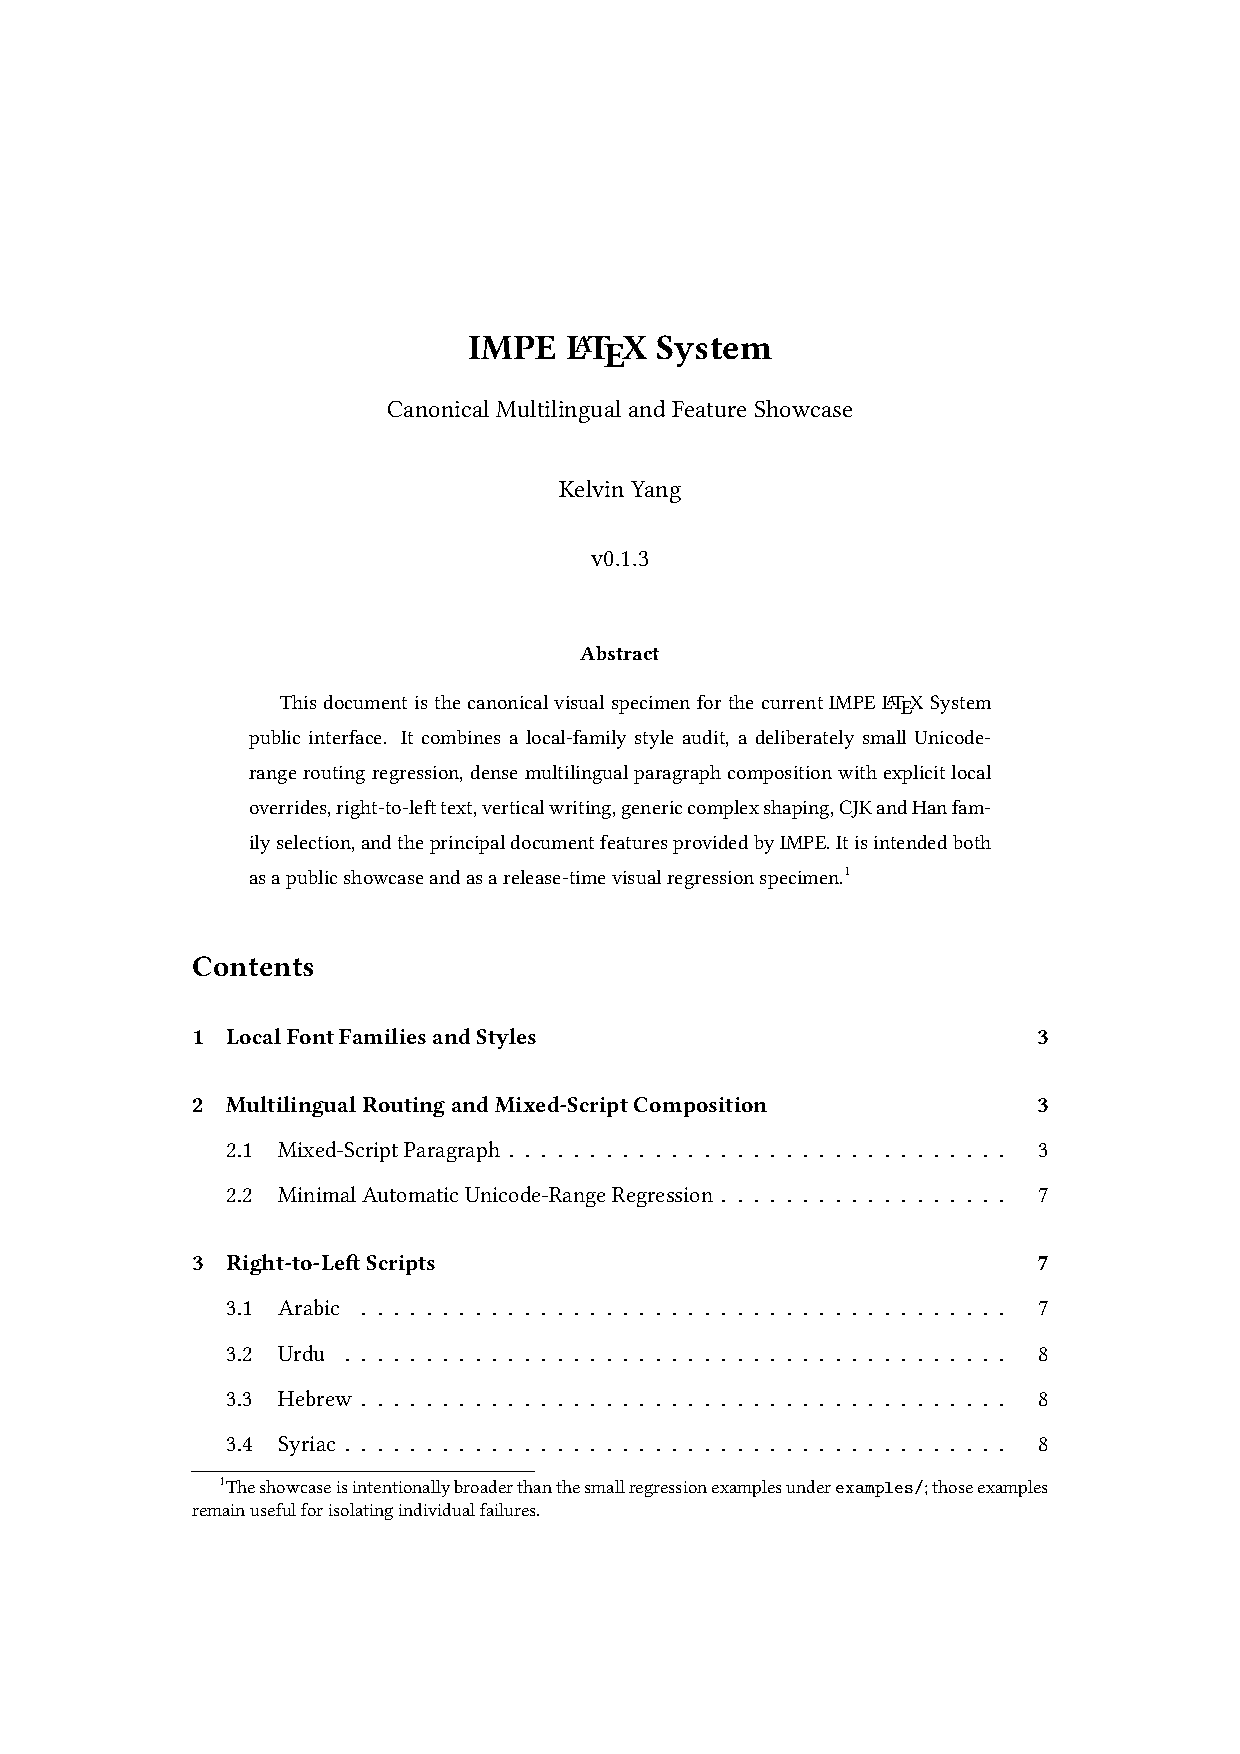
\includepdf[pages=-,pagecommand={}]{impe-showcase.pdf}}
  {\PackageError{impe-manual}
     {Required staged resource impe-showcase.pdf is missing}
     {Run scripts/build_manual.ps1 from the repository root.}}

\end{document}
